\documentclass{article}

\usepackage[parfill]{parskip}
\usepackage{graphicx}
\usepackage{amsmath}
\usepackage{tikz}
\usepackage[utf8]{inputenc} % For åäö

\title{"Catch and Throw" ball and beam process\\FRTN01 -- Real-Time Systems}
\author{
Mattias Fält -- faldt.mattias@gmail.com
\and
Lucas Jimbergsson -- lucas@jimbergsson.se
\and
Erik Nossborn -- eki.nossborn@gmail.com
\and
Iulia Stoica -- mariajstoica@gmail.com
}

\begin{document}
\maketitle
\newpage

\tableofcontents
\newpage

\section{Introduction // Mattias}
\label{sec:introduction}
% Should state the problem to be solved
The goal of this project is to control a "ball and beam" process (depicted in figure \ref{fig:process}) in a predetermined sequence of tasks:
\begin{itemize}
\item Dispatch a ball from a ball magazine and let the beam catch it.
\item Determine the weight of the ball (comparing with three predefined possible weights).
\item Depending on the weight do either of the following:
\begin{itemize}
\item \textbf{Small ball}: Let it roll into the little cup to the upper left of the beam.
\item \textbf{Medium ball}: Throw it into a basket on the floor.
\item \textbf{Large ball}: Simply drop it on the floor.
\end{itemize}
\end{itemize}
\begin{figure}
\centering
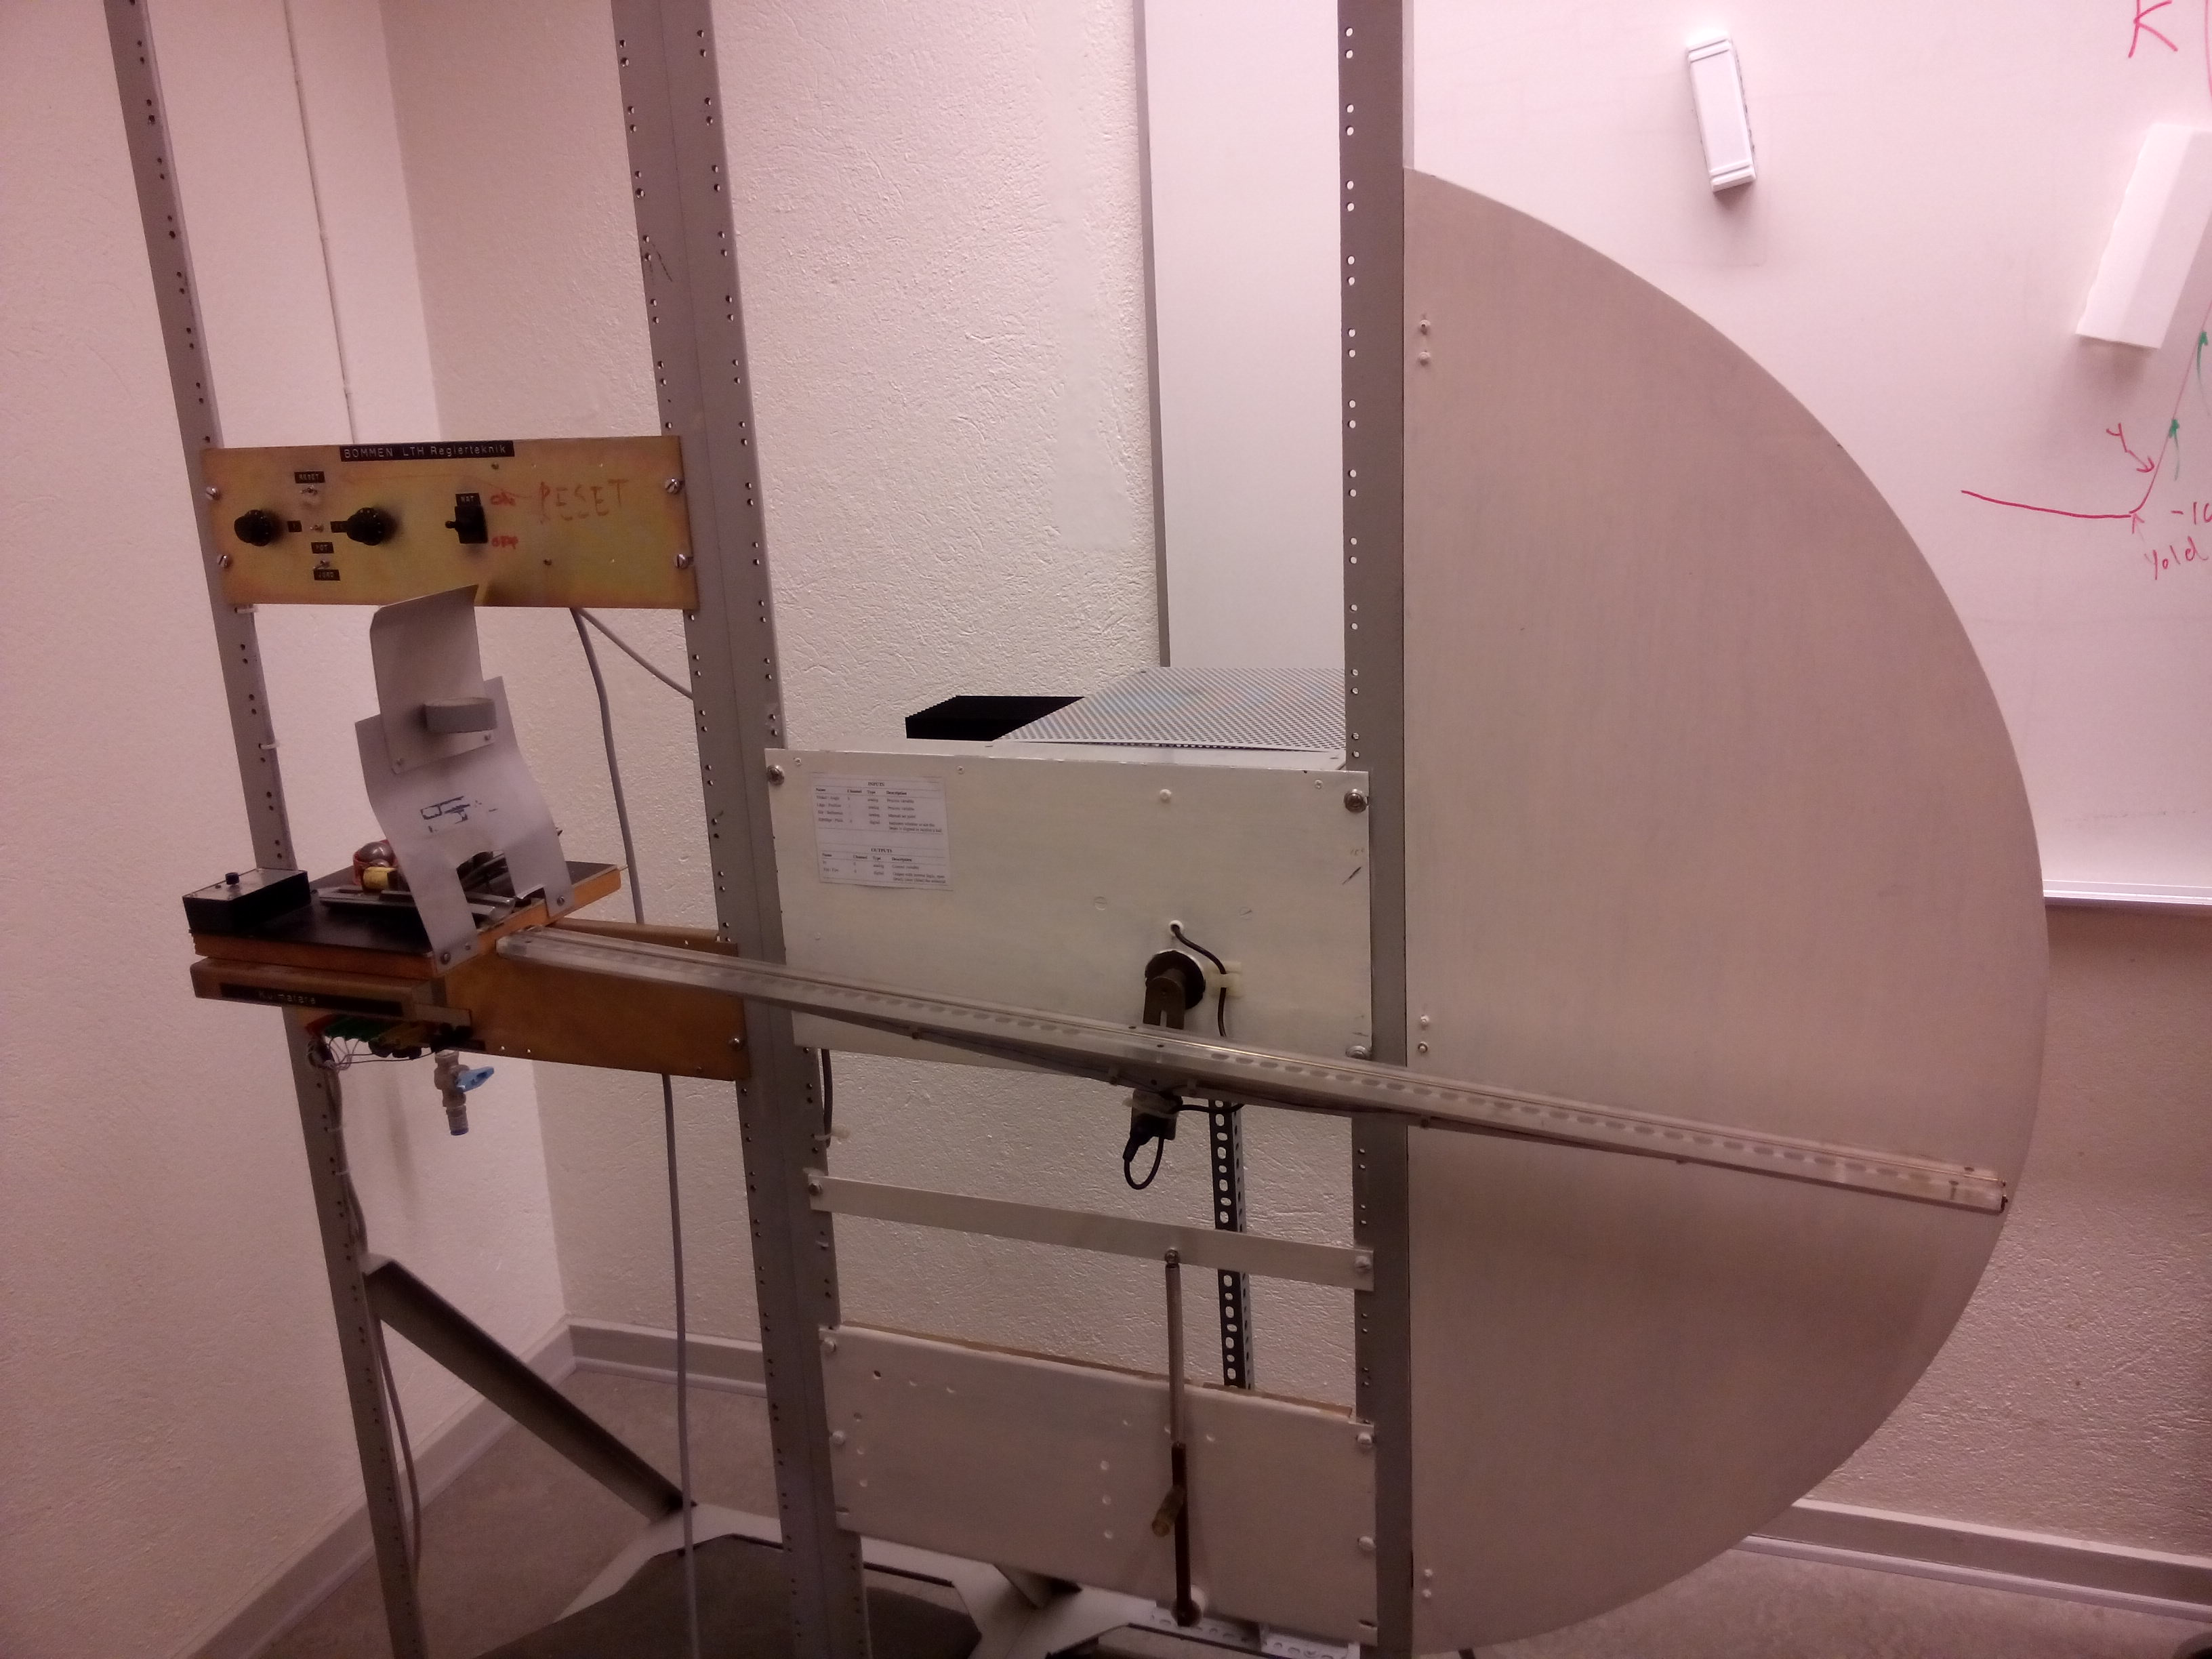
\includegraphics[width=0.7\textwidth]{figures/process_fig.jpg}
\caption{The "ball and beam" process to control.}\label{fig:process}
\end{figure}

\section{Overall approach //Mattias}
We initially intended on solving the control part of this project by generating trajectories for the ball and beam.
We would then use a time-varying LQG controller to stabilize the system around this predefined trajectory.
We generated the trajectories by iteratively improving the control signal using a gradient based optimization method.
We needed a model of the entire system for this to be possible, and although we did not end up using this method for controlling the system, we decided to include the model for completeness (see appendix \ref{sec:model}).
The main reason for not using this approach was that we knew that it should be possible to achieve satisfactory results using a cascaded PID controller with heuristically tuned references.
We thus chose the safer and possibly easier solution.


\section{Controller structure // Lucas} \label{sec:controller_structure}
% Should describe the control design aspects of the project.
When controlling the beam angle without any ball on the beam, we are using a simple PID controller.
When controlling the ball position along the beam, we are instead using a cascaded PID controller setup (see figure \ref{fig:cascaded_pid}).
Our implementation also allows for an additional beam angle reference to be supplied as a feed forward signal if desired, but in our final setup we do not make use of this.
\begin{figure}
\centering
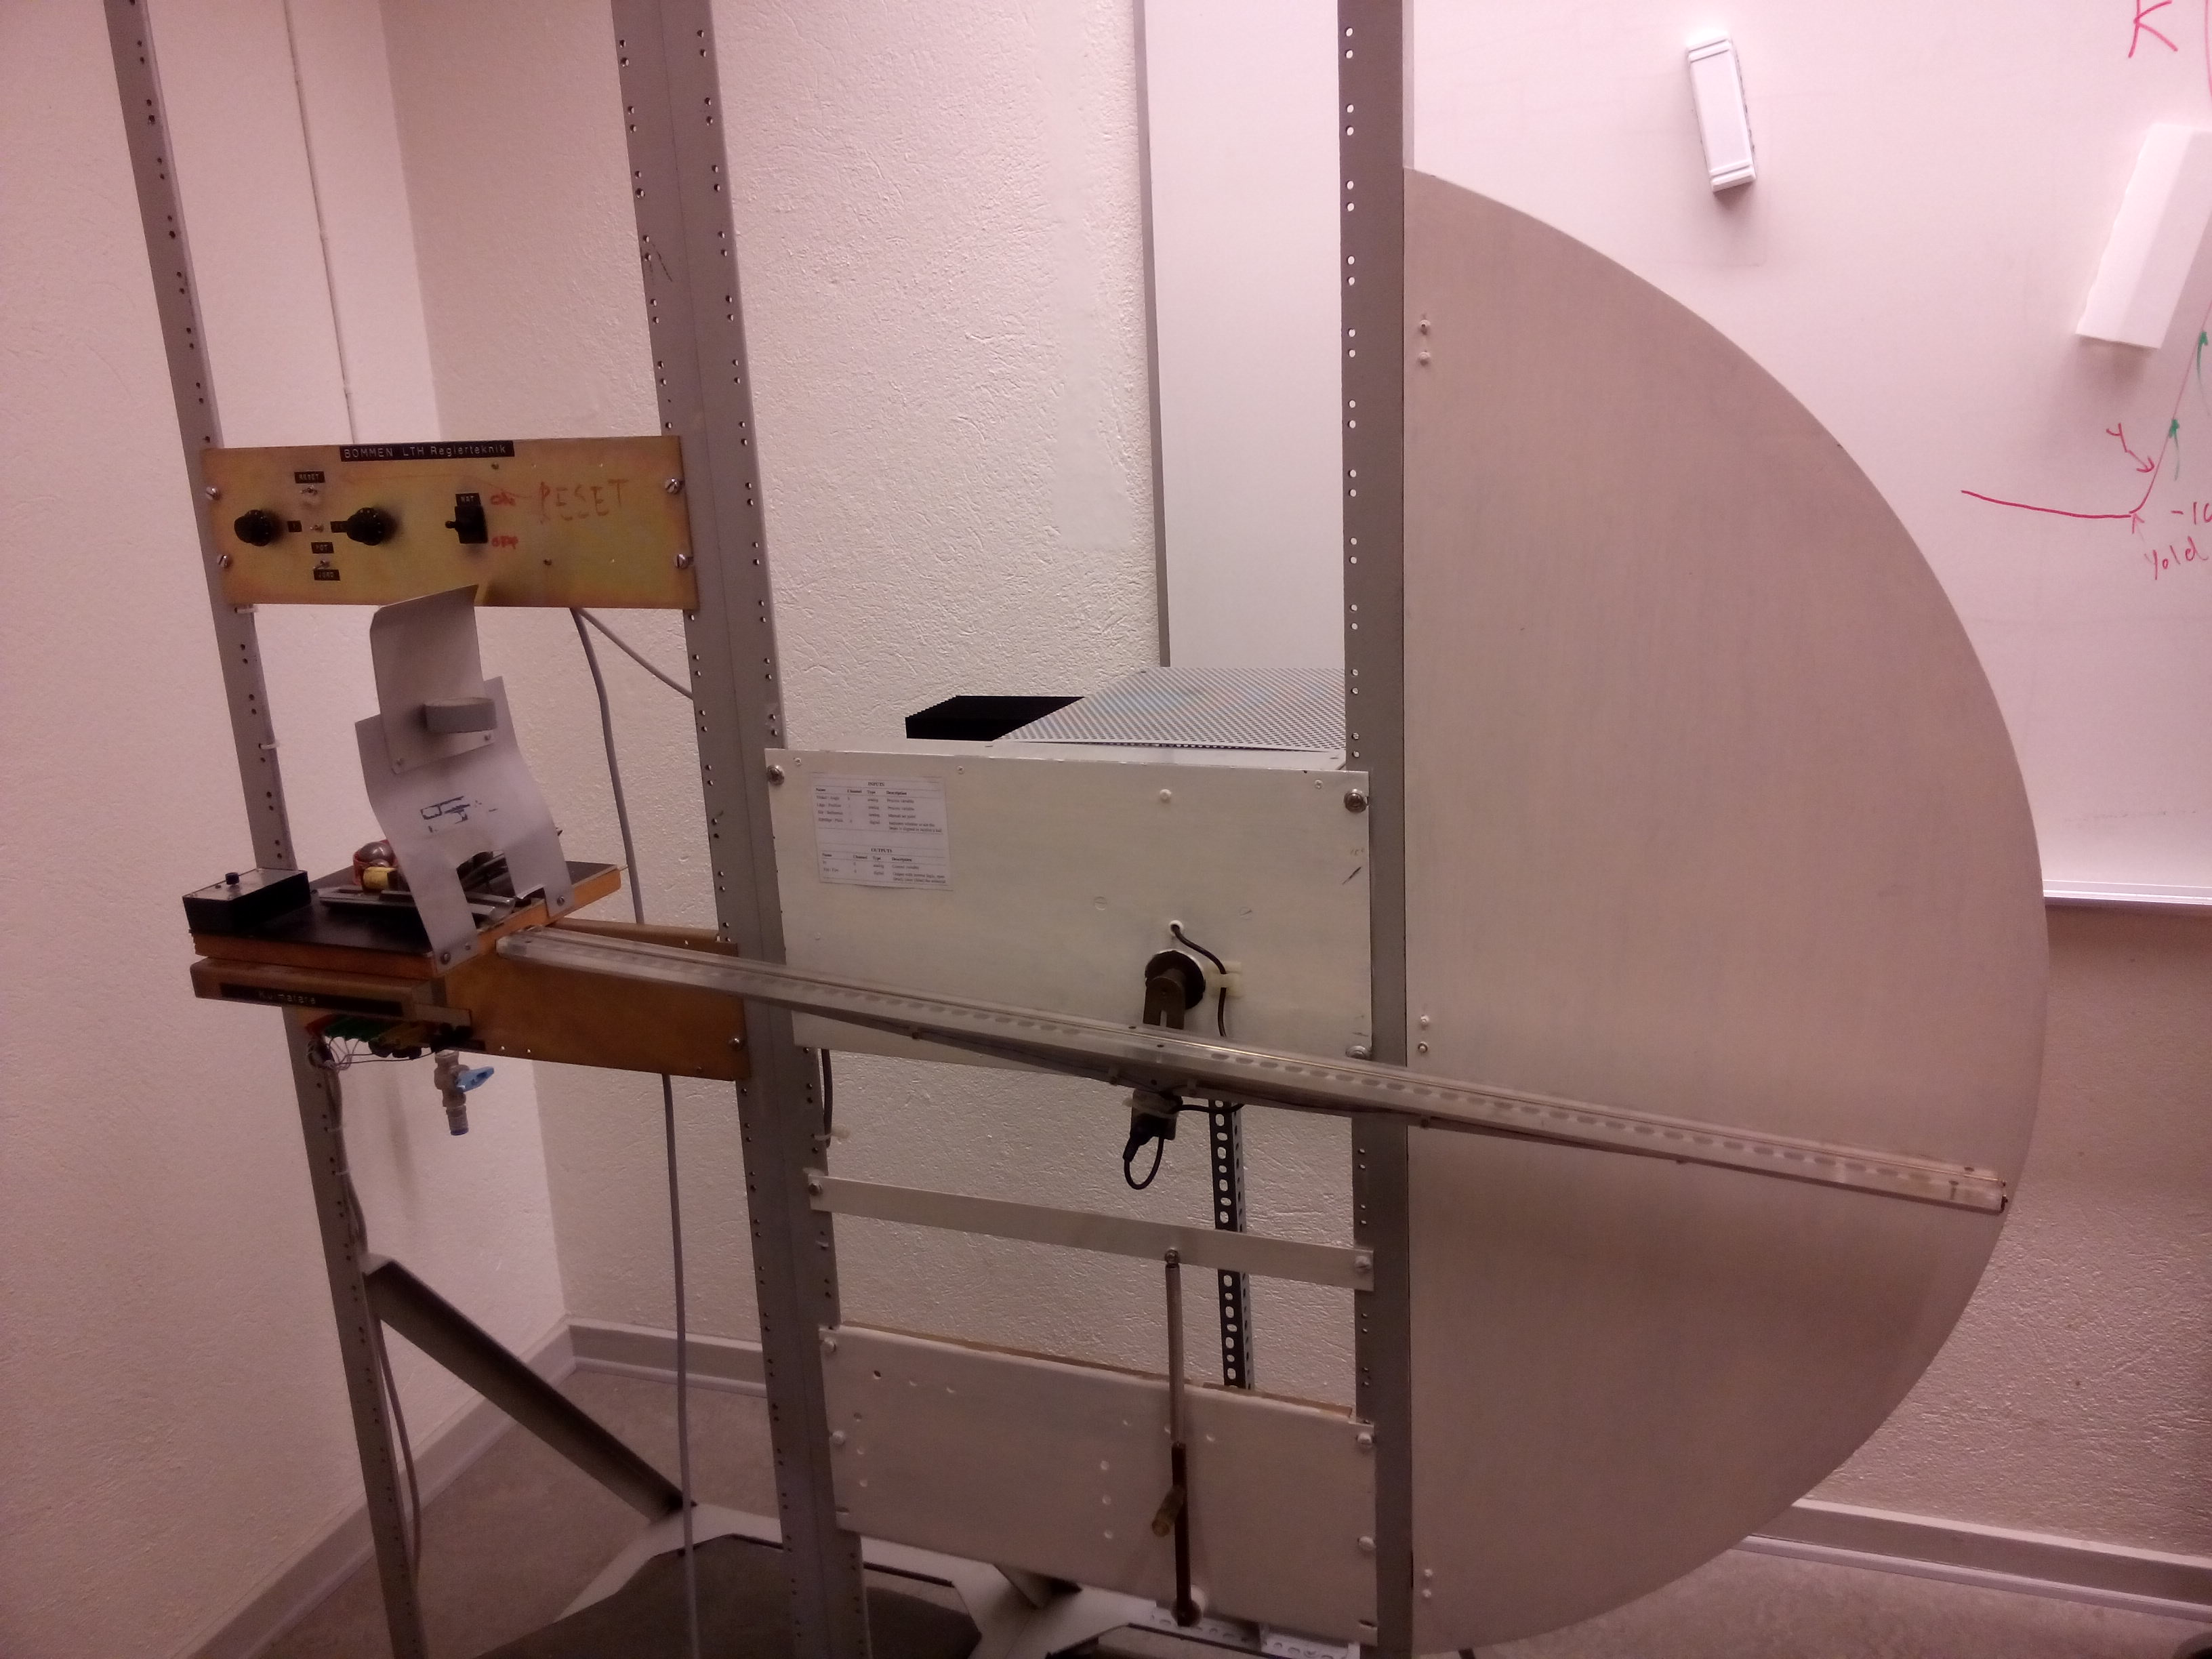
\includegraphics[width=0.7\textwidth]{figures/process_fig.jpg}
\caption{?????????????FIX BLOCK DIAGRAM???????????????The cascaded PID setup.}\label{fig:cascaded_pid}
\end{figure}

As mentioned in the introduction, we have a sequence of tasks to be performed, and each of these (catching, weighing and delivering the ball) will be described in further detail in the following sections.

\subsection{Ball catching}\label{sec:ball_catching}
The ball magazine shown to the left of the beam in figure \ref{fig:process} is equipped with a ball dispatcher solenoid, which can be controlled from our program in order to push away a ball from the magazine.
For the ball to roll onto the beam however, the beam has to be aligned with the dispatcher.

Since the sensor measuring the beam angle is not very reliable, we make use of an additional optical sensor detecting when the beam is aligned with the dispatcher.
Starting at some underestimated angle near the dispatcher, the search for the correct beam angle is done by slowly increasing the beam angle until the optical sensor triggers. A small beam angle bias is then corrected for dispatching a ball.

\subsection{Ball weighing}\label{sec:ball_weighing}
When the ball rolls onto the beam (from the left), we want to determine its weight by measuring how much control signal\footnote{The control signal is essentially corresponding to a motor torque applied on the beam.} is necessary for keeping the ball near a certain weighing position.
We choose the weighing position to be to the right on the beam, and when controlling the ball to this position we are careful to avoid the ball rolling off the beam.
This is achieved by setting the ball position reference signal to a slowly increasing ramp, ending up at the weighing position.

The torque on the beam caused by a ball's gravity force $mg$ is\footnote{We are ignoring that the rotational center of the beam not exactly at the mass centre of the ball when $x=0$, but actually slightly above.}
\[
\tau_{ball} = mgx
\]
where $x$ is the ball position. Letting $u$ denote the control signal, and assuming that $k_u u = \tau_{ball}$\footnote{The mass of the beam actually introduces an additional torque, since the beam is not rotating around its center of mass.
This can however be ignored for small beam angles, which is the case when balancing the ball at a certain position.} for some constant $k_u$, $mg/k_u$ can now be derived from $u$ and $x$.
Since $mg/k_u$ will always be the same for a particular ball, this measured quantity can now be used to indicate which ball is currently on the beam.

As the control signal $u$ can be very noisy, we apply lowpass filtering before deciding the ball size.
We are not as picky regarding the ball position however.
As $mg/k_u$ can be measured for any $x$, we do not need to wait for the controller to keep the ball entirely still at the weighing position before making the ball size decision.
This is implemented by having a high tolerance for the ball position, and reduces the running time of the weighing a lot.

\subsection{Ball delivery}\label{sec:ball_delivery}
Depending on the detected ball size, we now do different things according to the problem formulation in section \ref{sec:introduction}, explained in more detail in the following sections.

\subsubsection{Small ball}\label{sec:small_ball_delivery}
For the small ball to be rolled into the cup to the upper left from the beam, the ball is first stabilized at the weighing position in order to make the following actions more deterministic.
When stabilizing the ball, the tolerance is now much less as compared to when weighing.

After the ball is stabilized a heuristically pre-tuned angle reference trajectory (see figure \ref{fig:weighandthrowsmallball}) is applied, making the ball roll into the cup.
No ball position feedback is used.

\subsubsection{Medium ball}\label{sec:medium_ball_delivery}
POSITIONEN TILL VÄNSTER KALLAS THROWING POSITION \\

\subsubsection{Large ball}\label{sec:large_ball_delivery}
If the ball size is determined to be the largest one, a constant beam angle reference is simply applied, making the beam tilt and dropping the ball on the floor.




\section{Program structure //Erik}
% Should describe the main program structure, both from a class and and a real-time perspective. If possible illustrate this with some type of figure.
%Vad blir en bra ordning på rubrikerna? Är rubrikerna bra? lekte lite med ordningen på rubrikerna så att klasserna som beskrivs i varje rubrik har nämnts i texten/rubriken innan, vet inte om det är bra
%bytte plats så att trådarna beskrivs sist, för det är inte förrän där vi beskriver var varje klass faktiskt används. Då är det bra att ha sett vilka sorts klasser det finns. -E
%hur ska vi göra med klasser vi inte skrivit?



The program consists of two threads involved in the control, called \texttt{RegulThread} and \texttt{SwitchThread}, and one \texttt{Monitor} class for the synchronization of their work. 
\texttt{SwitchThread} has the task of switching between controller, reference generator and checker objects in the monitor. By setting these objects the thread gives the command to the \texttt{RegulThread} to perform control with the help of the current controller and reference generator until some desired state specified by the checker object is achieved. The switching thread is going to sleep and it is woken up when the conditions are fullfilled to give new commands.
\texttt{RegulThread} has then the task of calculating a control signal each sample, send it to the process and check if the desired state is achieved, see figure \ref{overall_fig}. How these tasks are performed is described in more detail in this chapter.

As mentioned before the synchronization needed when a switch is made is handled by the monitor and the monitor also handles some scheduling in the sense that it puts the \texttt{SwitchThread} to sleep and wakes it up when it is needed again.
The monitor is one of the central parts of the code and offers synchronization for other tasks too which will be described bellow in the context of each class using it. 
\begin{figure}
\centering
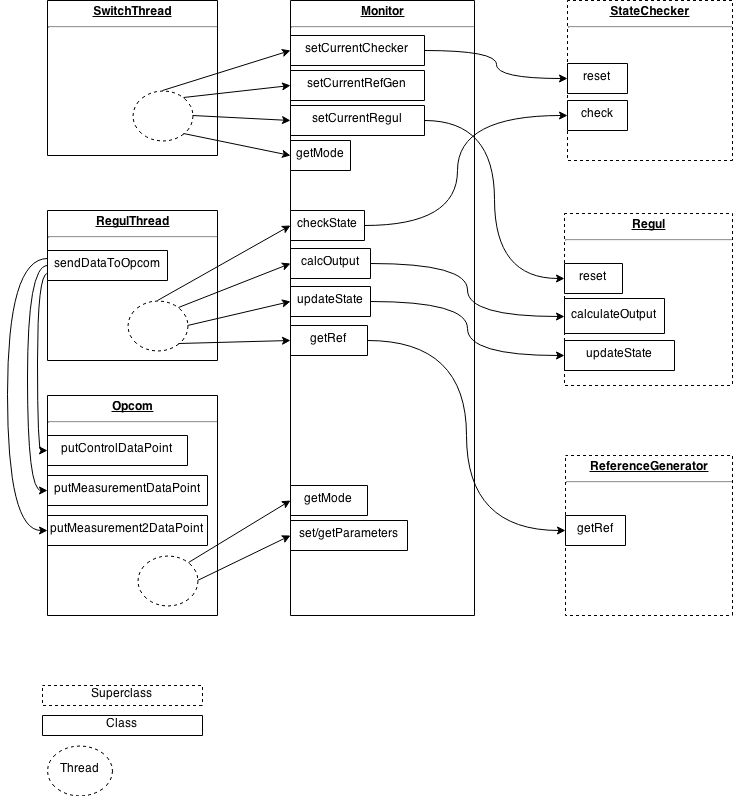
\includegraphics[width=\textwidth]{figures/UML.png}
\caption{UML of the code structure showing the classes and threads. For readability reasons superclasses are shown but not their subclasses. Some of the method names are fictive for example the method \texttt{setCurrentRegul} is referring to all the methods in the actual code that set a value to the current controller, one for each controller type}
\label{overall_fig}
\end{figure}

A few classes are not described below, as they are help classes that don't do much on their own. %kanske bara nämna vilka när vi vet vad vi faktiskt skrivit om... Tror det är PIDParameters och PlotData (och kanske OutSignal, men den kanske inte används alls)



%--------------------MISC CLASSES-----------------



\subsection{Miscellaneous classes} 	%Beskrivning av klasser som inte passar in under andra rubriker, tex Main och OpCom
%tror även Monitor bör få en snabb beskrivning här, men de flesta metoder i monitorn bör förklaras i beskrivningen av de klasser som faktiskt använder dem.
These classes don't fit under any other topic. They are found in the \texttt{main} package.

\subsubsection{Main.java}
%behöver nog inte beskrivas så ingående
This is the entry point of the program. 
All necessary objects are created, including the \texttt{Monitor}, the GUI, and all the threads.  
Once everything is set up, the threads are also started. 

\subsubsection{Monitor.java}
%behöver nog inte heller beskrivas så ingående här, bättre att skriva om den utifrån hur trådarna använder den.
This class provides sychronization between threads. Most calls to regulators and similar are done through the monitor. 
As such, the actual methods of the monitor are not very interesting in the context of this class, but rather in the context of the threads that invoke them. 
They will therefore be covered in section \ref{Threads} where the threads are described.

The monitor also has a lot of getters and setters, for variables that need synchronization across threads.

\subsubsection{OpCom.java}
%inte så ingående heller. Vi skrev den inte, och hur den funkar beskrivs nog bättre i Operator communication.
This is a slightly modified version of \texttt{OpCom} from Lab 1. 
The actual functionality will be described in section \ref{OpCom}. 
It communicates with the monitor, mostly through the \texttt{void set*Mode()} synchronized methods.



%--------------------REGULATORS-----------------




\subsection{Regulator classes}
Regulator classes determine how the control signal should be calculated, given measured states and reference values. 
They are found in the \texttt{regul} package.

\subsubsection{Regul.java}
This is the abstract superclass of all regulators. 
It has the abstract methods \texttt{calculateOutput}, \texttt{updateState} and \texttt{reset}.

\texttt{double calculateOutput(double[] measurement, double[] ref, double h)} takes the measured values, the reference values, and the period $h$ and calculates a desired control signal depending on the implementation in subclasses.

\texttt{void updateState(double h)} updates all the values that need updating before the next sample, but aren't needed to calculate the control signal for the current sample. 
This method is called after sending the control signal to the process, to minimize the delay between input and output.

The method \texttt{void reset(double[] states)} is used to reset the regulator after it has been activated, so it has relevant internal values that fit the current state of the system.

\subsubsection{BeamRegul.java}
\texttt{BeamRegul} is a PID regulator for controlling the angle of the beam. 
In addition to the implementations of the abstract methods, it also has a getter and a setter for the parameters (described by a \texttt{PIDParameters} object).

\subsubsection{BeamBallRegul.java}
This subclass is a cascaded PID regulator for controlling the position of the ball. 
It is like \texttt{BeamRegul}, except it also has a reference to a \texttt{BeamRegul} object inside itself. 
In this way, we get a simple way of describing a cascaded PID regulator. 
When calculating the control signal, this class calls the \texttt{calculateOutput} of its inner regulator. 
The same goes for updating and reseting.

%Vet inte vilka andra regulatorer som faktiskt används... Tror det bara är de där två ^



%--------------------REFERENCE GENERATORS-----------------




\subsection{Reference generator classes}
Reference generators are classes that determine where the reference values for the process should be at a particular point in time. 
Whenever a reference value is needed, it is requested from the currently chosen reference generator  (through a call to a monitor method). 
These classes are found in the \texttt{refgen} package.
 
\subsubsection{ReferenceGenerator.java}
This is the abstract superclass of the reference generators, and has the methods \texttt{double[] getRef()}, \texttt{void resetTime()} and \texttt{double getTimeSeconds()}.

\texttt{getRef()} must be implemented in subclasses, and is meant to return the current reference value.


\texttt{resetTime()} sets the starting time of the reference generator to the current time, essentially "resetting" it. 
Called whenever a reference generator is selected, but not relevant for time invariant subclasses.
%Inte säker på om denna metod används längre (av någon anledning), så isåfall bör den tas bort.
\texttt{getTimeSeconds()} gives the time in seconds since \texttt{resetTime()} was last called. 
Again not relevant for time invariant generators.

\subsubsection{ConstantRef.java}
This subclass gives a constant reference value chosen by calling \texttt{setRef(double)}. 
Which state the reference in an instance of this class refers to is given by the private variable \texttt{actualState} which is sent to the constructor at the creation of the object.

%\subsubsection{ConstantVectorRef.java}
%%Används denna?
%This class works the same as \texttt{ConstantRef}, but gives references to all states of the system.
%
%\subsubsection{ConstPosRampAngleRef.java}
%%används denna?

\subsubsection{RampRef.java}
\texttt{RampRef} gives a reference that changes linearly over time, and includes methods to set the slope and initial reference. 
Like in \texttt{ConstantRef}, a variable is used to determine which state the reference value in the current instance of the class refers to.

\subsubsection{RampToRef.java}
This subclass works almost like \texttt{RampRef}, except it stops when a chosen reference value has been reached. 
This gives a smoother reference change.

\subsubsection{RefGenGUI.java}
This is a slightly modified version of the \texttt{ReferenceGenerator} found in Lab 1, and was used for testing.

%\subsubsection{TrajectoryRef}
%%används denna?
%This subclass gives a reference that follows a curve loaded from a Matlab file.



%--------------------CHECKERS-----------------




\subsection{Checker classes}\label{Checkers}
Checker classes provide a method to determine if a state is "OK" in some way. 
We use this to find out when we should continue to the next part of the catch-throw sequence. 
These classes are found in the \texttt{checker} package.
\subsubsection{StateChecker.java}
\texttt{StateChecker} is the abstract superclass of all the checkers. It has two methods.

The method \texttt{boolean check(double[] measurement)} receives our measured values and returns a boolean describing if the state of the system fulfills some condition, depending on the implementation in subclasses.

\texttt{void reset()} is used when activating a checker to reset their internal states, so any previous usage of the object won't  affect the current workings. 
This method will be empty in subclasses that have no internal state.

%\subsubsection{BallOnBeamChecker.java}
%just nu använder vi inte den här, men det finns förändringar vi kan göra för att den ska funka

\subsubsection{ConstBallChecker.java}
This subclass checks if a ball has been around a specified point on the beam for a sufficient number of samples in a row. 
It provides the method \texttt{void setValue(double y, double tol)} for choosing the wanted stationary point and needed precision.

\subsubsection{ConstBeamChecker.java}
Almost exactly the same as \texttt{ConstBallChecker}, except for the angle of the beam. 
It does, however, not have the ability to change the tolerance. 

\subsubsection{LEDChecker.java}
Checks if the beam is in the pickup position - in other words if the LED is on. 
This is done by actually reading the digital in channel.

\subsubsection{Null checker}
Though not a class, the monitor has the ability to set the "null checker", which is roughly equivalent to turning off checking. 
This is not needed, since calling a checker when SwitchThread is not waiting or ready to run does nothing except waste time, but it can avoid unneccesary processor load to some extent.




%--------------------THREADS-----------------




\subsection{Threads}\label{Threads}

\subsubsection{RegulThread.java}
This is the main regulator loop. Every loop iteration, this thread does the following things (in order):
\begin{itemize}
\item reads input from process
\item calculates output
\item sends output to process
\item sends data to the GUI
\item updates the state of the regulator
\item checks the state of the system
\end{itemize}

Except for reading and sending, these things are done by calling methods in \texttt{Monitor}. 
As such, their exact functionalities depend on which settings have been chosen in the monitor. 
This thread runs oblivious of changes to the settings, and has no need to know of them; the basic structure of the loop remains the same.

When the thread calls the synchronized method \texttt{double calcOutput(double[] measurement)}, the result is calculated using \texttt{currentRegul} in the monitor. 
Depending on monitor calls from other threads (namely \texttt{SwitchThread} and \texttt{OpCom}), the actual object \texttt{currentRegul} points to will be different. 
In the same way, the reference values needed to do the output calculations are received from \texttt{currentRefGen}, which also points to different objects depending on the wanted functionality.

"Checking" the state of the system means to evaluate if the system fulfils certain criteria. 
The actual criteria, again, depend on settings given to the monitor. 
If the state is deemed "ok", waiting threads (in our case, \texttt{SwitchThread}) are awoken. 
Otherwise, nothing happens. More details in sections \ref{SwitchThread} and \ref{Checkers}.



\subsubsection{SwitchThread.java}\label{SwitchThread}
\texttt{SwitchThread} is the thread that handles our sequence mode.

It uses monitor calls to change regulators and reference generators to modify the behaviour of the process. 
It also uses checker classes to wait for certain events to happen, or \texttt{Thread.sleep()} in case a certain amount of time needs to pass.

Changing of regulators is done through the \texttt{set*Regul()} monitor methods, while reference generators are set through the \texttt{setRefGen*()} methods. 
In the reference generator case, the arguments are different depending on the reference generator. 
Changing of regulators and reference generators is generally done within a single synchronized block.

When the thread calls the synchronized methods \texttt{void set*Check}, where \texttt{*} and arguments depend on the particular checker wanted, the monitor's \texttt{stateChecker} is set to an instance of the wanted checker, the relevant settings in the chosen checker are set, and the thread calls \texttt{wait()}. 
The responsibility of waking this thread up now falls to \texttt{RegulThread}, which polls the currently selected checker every iteration. 
If the polled checker returns \texttt{true}, it wakes all waiting threads up, allowing \texttt{SwitchThread} to continue executing. 
In this way, this thread knows the state of the system is satisfactory to continue with the sequence once it wakes up.

The thread can also wake up if sequence mode is turned off, in which case the thread will go back to the starting position and wait to be turned on again.

This thread also handles the digital output, shooting out a ball when the process is ready to receive it.

The general structure of a segment is
\begin{itemize}
\item set a regulator,
\item set a reference generator,
\item set a checker and wait to wake up
\end{itemize}

Of course, the different parts need to go together: if you set the regulator to regulating the beam, 
the reference generator should also give a reference for the beam, 
and the checker needs to wait for a state that will actually be achieved.

After the ball has been weighed, the checkers are no longer used, and instead beam angle changes in combination with sleeps handle the throwing.



\section{Operator communication //Iulia}\label{OpCom}
% Should describe the user interface in the project including a short HowTo description on how to start and operate the program.
The program is started by running the \texttt{Main} class which can be found in the \texttt{main} package and the user interface should pop up shortly.

The user interface consists of a main window called "Ball and beam GUI" which contains three realtime graphs where the upper one and the middle one are plotting the reference values (in black) and measurements (in red) for the beam and the ball respectively and the last one is plotting the control signal. The window also contains two fields where one can change the parameters of the controller for the beam's angle and the ball's position online and also a set of buttons which can change the running mode of the program:
\begin{itemize}
\item mode OFF: the controllers are off
\item mode BEAM: the program is running control of the beam's angle only and the user can change the reference value manually
\item mode BALL: the program is running control of both the beam's angle and the ball's position and the user can change the reference values manually
\item mode Sequence: the program is running sequence until stopped, i.e catch a ball, weigh the ball, throw the ball and get ready for another sequence
\end{itemize}

The user interface also contains two smaller windows called "Angle RefGen" and "Position RefGen" where the user can change the reference values of the beam's angle and the ball's position when the program is running in one of the manual modes, i.e BEAM or BALL mode.
\section{Results //Erik}
% A section containing the results. In case the project is a control-oriented project this should include plots of measurement signals, reference signal, and control signal. If the project is more of a real-time nature then this section could contain measurement results of different type.

%PLOTTAR FÖR SEQUENCE, FÖRKLARA NÄR VAD HÄNDER \\
%klart, eller?
FÅ PLOTTAR ATT LIGGA RÄTT I DOKUMENTET

In the figures, the top graph shows the reference values and measured values for the angle of the beam. 
The middle graph shows the same values for the position of the ball. 
Reference values are shown in black, while measured values are red. 
The bottom plot shows the control signal.

Figures \ref{fig:stepresponsebeam} and \ref{fig:stepresponseball} show the step responses for the beam angle and the ball position, respectively. 
The beam step response shows a large overshoot but a quick settling.
The ball step response also shows a quite large overshoot, while also being quite slow.
As the plots show, the control signal has a tendency to be noisy.

Figures \ref{fig:topickupposition}-\ref{fig:weighbandthrowlargeball} show plots for different parts of the sequence described in Section \ref{sec:controller_structure}.
As can be seen in for example Figure \ref{fig:weighmediumball}, no great precision is needed when weighing the ball. See Section \ref{sec:ball_weighing}.

\begin{figure}[h]
\centering
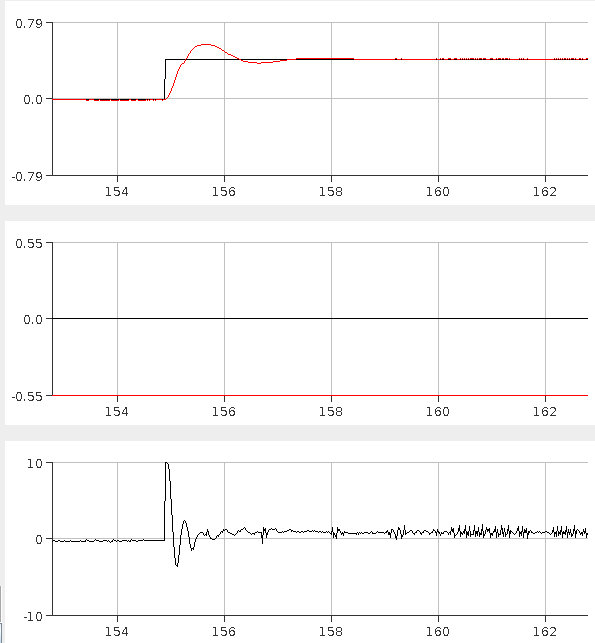
\includegraphics[width=0.7\textwidth]{figures/stepresponsebeam-crop.png}
\caption{Step response for the beam angle.}
\label{fig:stepresponsebeam}
\end{figure}

\begin{figure}[h]
\centering
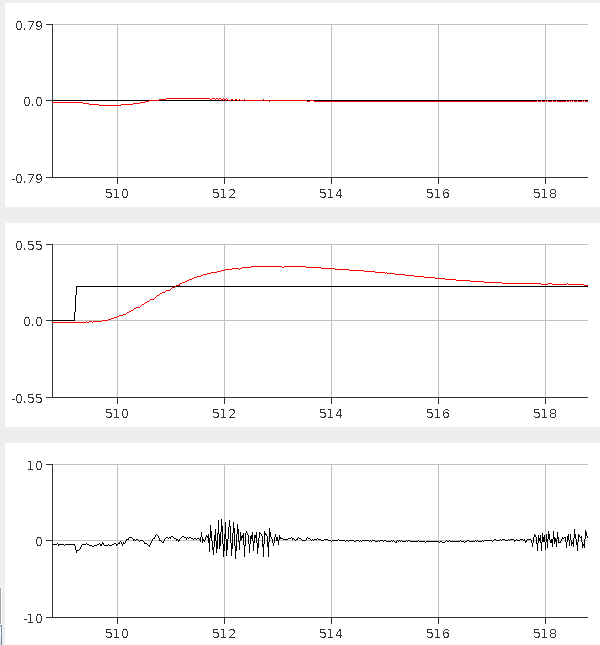
\includegraphics[width=0.7\textwidth]{figures/stepresponseball1-crop.png}
\caption{Step response for the ball position. Notice the noisy control signal.}
\label{fig:stepresponseball}
\end{figure}

\begin{figure}[h]
\centering
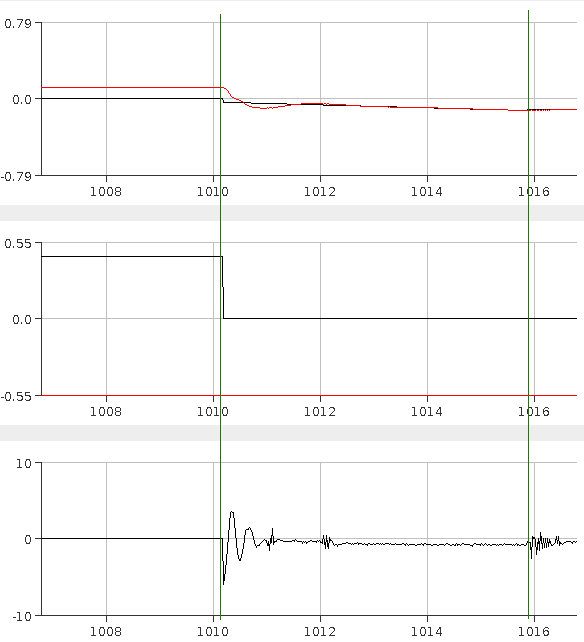
\includegraphics[width=0.7\textwidth]{figures/topickupposition-crop.png}
\caption{Controlling the beam angle to search for the appropriate pickup position, as described in Section \ref{sec:ball_catching}. The process is started at the first line in the graph, and the LED is detected around the second.}
\label{fig:topickupposition}
\end{figure}

\begin{figure}[h]
\centering
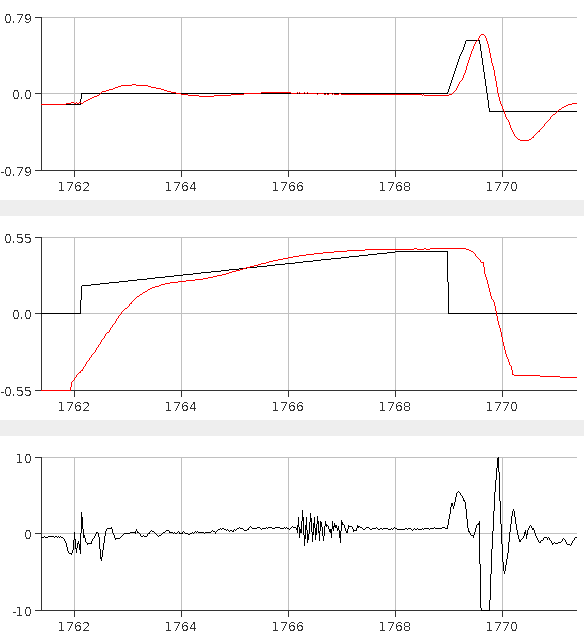
\includegraphics[width=0.7\textwidth]{figures/weighandthrowsmallball-crop.png}
\caption{Weighing and throwing the small ball. The ball enters the beam at the first line, and is finished being weighed around the second one. After being stabilized (See Section \ref{sec:small_ball_delivery}), it is thrown at the third line.}
\label{fig:weighandthrowsmallball}
\end{figure}

\begin{figure}[h]
\centering
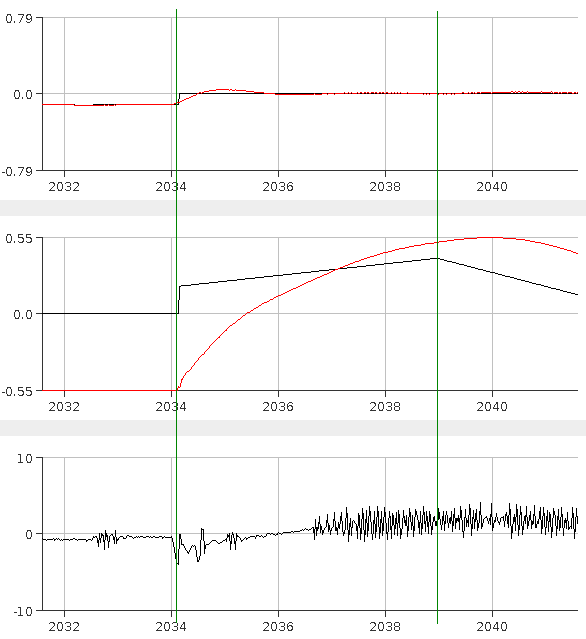
\includegraphics[width=0.7\textwidth]{figures/weighmediumball-crop.png}
\caption{Weighing the medium ball, and the beginning of moving it to prepare for a throw. The ball is detected at the first line, and is finished being weighed at the second.}
\label{fig:weighmediumball}
\end{figure}

%kanske inte jätteintressant?
\begin{figure}[h]
\centering
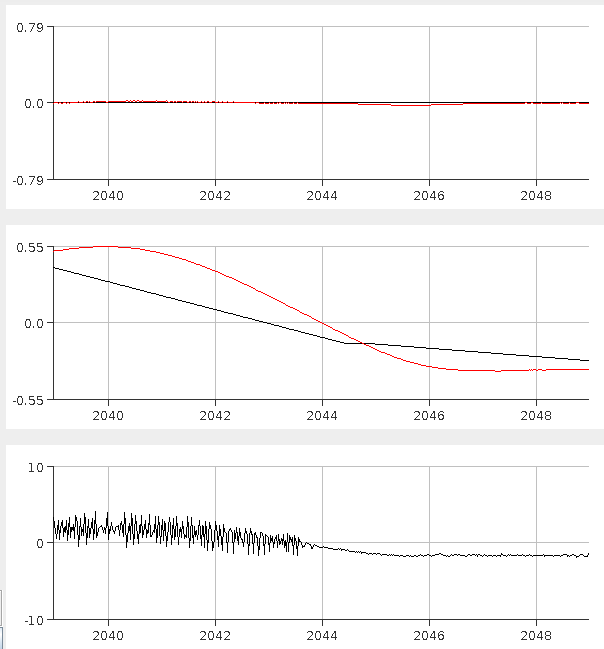
\includegraphics[width=0.7\textwidth]{figures/movemediumball-crop.png}
\caption{Moving the medium ball to throwing position.}
\label{fig:movemediumball}
\end{figure}

\begin{figure}[h]
\centering
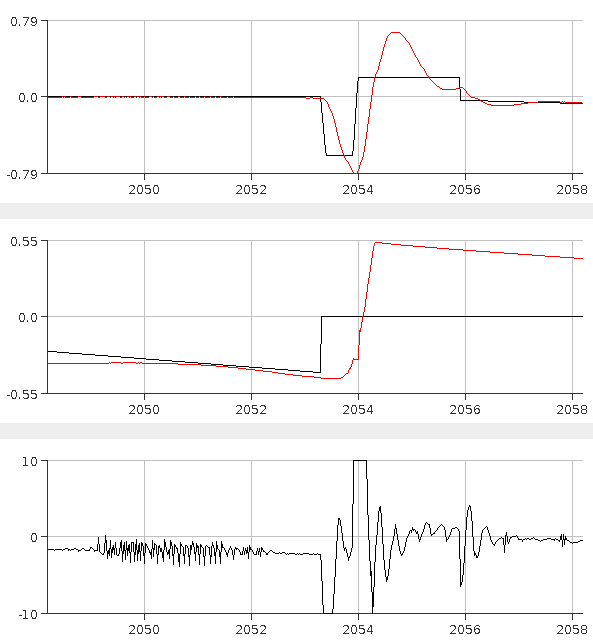
\includegraphics[width=0.7\textwidth]{figures/throwmediumball-crop.png}
\caption{The medium ball arriving at the throwing position, and then getting thrown, at the time point specified by the line.}
\label{fig:throwmediumball}
\end{figure}

\begin{figure}[h]
\centering
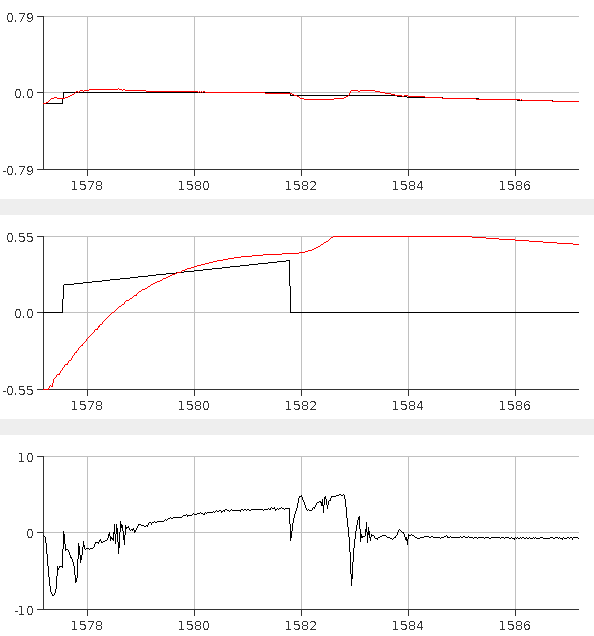
\includegraphics[width=0.7\textwidth]{figures/weighanddroplargeball-crop.png}
\caption{Weighing and dropping the large ball. The ball enters the beam at the first line, and is finished being weighed at the second, after which it is dropped.}
\label{fig:weighbandthrowlargeball}
\end{figure}





\section{Conclusions //Lucas}

\subsection{Controller performance}
As seen in the step response in Figure \ref{fig:stepresponsebeam}, the beam control works well but is quite aggressive.
The controller being aggressive is mainly due to heavy integral action.
This is a deliberate choice of ours, in order to manage balancing even the largest ball with acceptable performance.

For the ball, the step response (see Figure \ref{fig:stepresponseball}) takes much more time to settle.
These differences in behaviour are to be expected, since the ball balancing problem is much harder.
Ball balancing being harder is partly because the ball dynamics are unstable, and partly because we are actually dealing with one control problem on top of another.
The quite large overshoot in the ball step response could possibly have been reduced, but probably at the price of problems with stationary errors (induced mainly by small "wells" on the beam, in which the ball can get stuck).

The control signal being noisy (as seen in the ball step response in Figure \ref{fig:stepresponseball}, for instance), seem to be caused by noisy measurement signals together with derivative action in the PID-controllers.
For both of these the derivative is lowpass-filtered, and we have been experimenting with the level of smoothing. If the derivative is smoothed too much however, the controller gets a slower response to ball/beam accelerations.
The spurious behaviour of the control signal being noisy or not is harder to explain.
One possibility is that the measurements are sometimes more and sometimes less reliable.
For the ball, we have noticed that at som instants it does not get detected, resulting in a slowly decreasing measurement signal.

\subsection{Evaluation of selected approach}
The selected approach of PID controllers together with heuristically tuned references works over our expectations, since we did not even see it as an alternative in the beginning. Its simplicity (not having any explicit need of a process model for example) is also very appealing.

Our initial model-based approach of time-invariant LQG with numerically optimized state trajectories would however possibly have been more beautiful in its generality and.

Worth noting is also that the PID/heuristic approach has a strong coupling (one affecting the other) between changes in PID parameters and changes in references. For the LQG/trajectory approach however, the coupling between the choice of weight matrices and the choice of reference trajectory specifications would not have been as prominent.



\newpage
\begin{thebibliography}{9}
\bibitem{NR}
  Thomas Bewley,
  \emph{Numerical Renaissance: simulation, optimization, \& control}.
  Renaissance Press,
  http://numerical-renaissance.com/NR.pdf

\end{thebibliography}

\appendix

\section{Process model //Mattias}\label{sec:model}
\subsection{System Equations}


The equation for a ball on a beam was taken from the material from the first lab in the course, and can be written as

\begin{equation}
m(\ddot{x}-x\dot{\phi}^{2})=-mg\sin(\phi)-\frac{2}{5}m\ddot{x},
\end{equation}
where $x$ is the distance of the ball along the beam, $m$ is the mass of the ball and $\phi$ is the angle of the beam.

We chose a simple model for the beam, letting the control signal be proportional to the torque on the beam.
To account for the displacement of the beam around the rotational center, we modeled a force proportional to the angle of the beam.
This approximation turned out to be quite good, especially for small angles.
The last part of this model is the force applied to the beam by the ball.
The differential equation is given as
\begin{equation}
J_{B}\ddot{\phi}=k_{u}u+mgx\cos(\phi)+k_B\phi,
\end{equation}
where $J_{B}$ is the moment of inertia of the beam, $k_u$ is the torque to control signal ratio and $k_B$ the estimated torque per radian from the displacement of the beam.\\
\\
Letting $x_{1}=x,\, x_{2}=\dot{x},\, x_{3}=\phi,\, x_{4}=\dot{\phi}$,
we can then write the system as a set of first order nonlinear differential equations

%\begin{eqnarray*}
%m(\dot x_{2}-x_{1}x_{4}^{2}) & = & -mg\sin(x_{3})-\frac{2}{5}m\dot{x}_{2}\\
% & \Leftrightarrow\\
%\dot{x}_{2} & = & \frac{5}{7}\left(-g\sin(x_{3})+x_{1}x_{4}^{2}\right)
%\end{eqnarray*}
%
%
%and beam equation as
%\[
%\dot{x}_{4}=\frac{1}{J_B}\left(k_{u}u+mgx_{1}\cos(x_3)+k_Bx_3\right).
%\]
%
%
%We thus have then nonlinear first order system equations

\[
\begin{pmatrix}\dot{x}_{1}\\
\dot{x}_{2}\\
\dot{x}_{3}\\
\dot{x}_{4}
\end{pmatrix}=\begin{pmatrix}x_{2}\\
\frac{5}{7}\left(-g\sin(x_{3})+x_{1}x_{4}^{2}\right)\\
x_{4}\\
\frac{1}{J_B}mgx_{1}\cos(x_3)+\frac{k_B}{J_B}x_3
\end{pmatrix}+\begin{pmatrix}0\\
0\\
0\\
\frac{k_{u}}{J_B}
\end{pmatrix}u.
\]

\subsection{Linearization}

We introduced the mass of the ball as a state $x_{5}=m$ in the system. The advantage of this is that it would then be possible to start estimating the weight of the ball earlier in the sequence.
It would also allow feed forward to the control signal based on the mass and position of the ball, this could have greatly reduced the oscillations of the beam control since we would not require integral action to account for this entire force.
We lastly introduced the integral of the deviation of the position of the
ball $(\tilde{x}_{6}=\int_{0}^{t}\tilde{x}_{1}dt)$ as a state and linearized the system around the steady state $\bar{x}=(\bar{x}_{1},0,0,0,\bar{m},\bar{u})$.
This results in the linear perturbation equations
%\begin{eqnarray*}
%\dot{\tilde{x}} & = & \begin{pmatrix}0 & 1 & 0 & 0 & 0\\
%\frac{5}{7}\bar{x}_{4}^{2} & 0 & -\frac{5g}{7}\cos(\bar{x}_{3}) & 2\bar{x}_{1}\bar{x}_{4} & 0\\
%0 & 0 & 0 & 1 & 0\\
%\bar{m}\frac{g}{J_B}\cos(\bar{x}_{3}) & 0 & -\bar{m}\frac{g}{J_B}\bar{x}_{1}\sin(\bar{x}_{3})+\frac{k_B}{J_B} & 0 & \frac{g}{J_B}\bar{x}_{1}\cos(\bar{x}_{3})\\
%0 & 0 & 0 & 0 & 0
%\end{pmatrix}\tilde{x}+\begin{pmatrix}0\\
%0\\
%0\\
%\frac{k_{u}}{J_B}\\
%0
%\end{pmatrix}\tilde{u}\\
% & = & \begin{pmatrix}0 & 1 & 0 & 0 & 0\\
%0 & 0 & -\frac{5g}{7} & 0 & 0\\
%0 & 0 & 0 & 1 & 0\\
%\bar{m}\frac{g}{J_B} & 0 & \frac{k_B}{J_B} & 0 & \frac{g}{J}\bar{x}_{1}\\
%0 & 0 & 0 & 0 & 0
%\end{pmatrix}\tilde{x}+\begin{pmatrix}0\\
%0\\
%0\\
%\frac{k_{u}}{J_B}\\
%0
%\end{pmatrix}\tilde{u}.
%\end{eqnarray*}

\begin{eqnarray*}
\dot{\tilde{x}} & = & \begin{pmatrix}0 & 1 & 0 & 0 & 0 & 0\\
0 & 0 & -\frac{5g}{7} & 0 & 0 & 0\\
0 & 0 & 0 & 1 & 0 & 0\\
\bar{m}\frac{g}{J_B} & 0 & \frac{k_B}{J_B} & 0 & \frac{g}{J_B}\bar{x}_{1} & 0\\
0 & 0 & 0 & 0 & 0 & 0\\
1 & 0 & 0 & 0 & 0 & 0
\end{pmatrix}\tilde{x}+\begin{pmatrix}0\\
0\\
0\\
\frac{k_{u}}{J_B}\\
0\\
0
\end{pmatrix}\tilde{u}\\
 & = & A\tilde{x}+B\tilde{u}\\
\tilde{y} & = & \begin{pmatrix}1 & 0 & 0 & 0 & 0 & 0\\
0 & 0 & 1 & 0 & 0 & 0
\end{pmatrix}\tilde{x}+w=C\tilde{x}
\end{eqnarray*}
where $\tilde{x}=x-\bar{x}$, $\tilde{u}=u-\bar{u}$.
\\
The system is now in a form that works with the LQG framework.

%where $v$ and $w$ has intensity matrices $V$ and $W$. We now define
%the cost function $J=E\left[\int_{0}^{\infty}\tilde{x}^{T}Q\tilde{x}^{T}+u^{T}\frac{1}{r^{2}}u\, dt\right]$,
%with $Q=\text{diag}\left(\frac{1}{q_{1}^{2}},\frac{1}{q_{2}^{2}},\frac{1}{q_{3}^{2}},\frac{1}{q_{4}^{2}},\frac{1}{q_{5}^{2}}\right)$
%and let the controller be

%\begin{eqnarray*}
%\dot{\hat{x}} & = & A\hat{x}+B\tilde{u}+K(y-C\hat{x})\\
%\tilde{u} & = & -L\hat{x}.
%\end{eqnarray*}


%The optimal $K$ and $L$ is then given by the symmetric positive
%definite solutions $P$ and $S$ to 
%\begin{eqnarray*}
%0 & = & AP+PA^{T}-PC^TW^{-1}CP+V\\
%0 & = & A^{T}S+SA-SBR^{-1}B^{T}S+Q
%\end{eqnarray*}


%as $K=PC^{T}W^{-1}$ and $L=R^{-1}B^{T}S$.

%An initial guess for the matrices $Q$ and $R$ could be given by
%giving similar penalty for deviations $(3cm,1cm/s,2^{\circ},0.5^{\circ}/s,-,20cm\cdot s)$
%and $(1V)??$. Thus

%$Q=\text{diag}(1111,10000,816,13131,0,25)$, $R=1.$


\subsection{Throw Equations}

To be able to throw the ball to a desired location we needed to know how the relation between the terminal state of the ball on the beam and the distance traveled in the air.
We derived this relation using the nonlinear system equations above and the equations for a free falling body.
The resulting equations are

%\begin{eqnarray*}
%h & = & h_{0}+v_{y_{0}}t-\frac{gt^{2}}{2}\\
%d & = & d_{0}+v_{x_{0}}t,
%\end{eqnarray*}


%which results in the terminal time $t_{T}=(d_{T}-d_{0})/v_{x_{0}}$.

%We desire 
%\begin{eqnarray*}
%h_{T} & = & -d_{y}\\
%d_{T} & = & d_{x},
%\end{eqnarray*}


%and know
%\begin{eqnarray*}
%h_{0} & = & l\sin(\phi)\\
%d_{0} & = & l\cos(\phi),
%\end{eqnarray*}


%which gives
%\begin{eqnarray*}
%-d_{y} & = & l\sin(\phi)+v_{y_{0}}t-\frac{gt^{2}}{2}\\
%d_{x} & = & l\cos(\phi)+v_{x_{0}}t.
%\end{eqnarray*}


%The velocity of the ball in the horizontal and vertical directions
%are
%\begin{eqnarray*}
%v_{x} & = & \dot{x}\cos(\phi)-x\dot{\phi}\sin(\phi)\\
%v_{y} & = & \dot{x}\sin(\phi)-x\dot{\phi}\cos(\phi),
%\end{eqnarray*}


%and at the release-time, we have $x=l$. These equations gives
\begin{eqnarray*}
-d_{y}(t) & = & l\sin(\phi)+\left(\dot{x}\sin(\phi)-l\dot{\phi}\cos(\phi)\right)t-\frac{gt^{2}}{2}\\
d_{x}(t) & = & l\cos(\phi)+\left(\dot{x}\cos(\phi)-l\dot{\phi}\sin(\phi)\right)t,
\end{eqnarray*}
where $d_{y}(t), d_{x}(t)$ are the distances traveled after time $t$ as given in Figure \ref{fig:throw} and $(x=l,\dot x,\phi, \dot{\phi})$ is the state when the ball is leaving the beam.

\begin{figure}[\textwidth]
\centering
\begin{tikzpicture}[scale=1.5]
\usetikzlibrary{patterns,snakes}
\definecolor{Darkgreen}{rgb}{0,0.4,0}
\tikzstyle{brace} = [decorate, decoration={brace, amplitude=5pt}]

\node[inner sep=0] (v0) at (0,0) {};
\node[inner sep=0] (v2) at (2,0.5) {};
\node[inner sep=0] (v1) at (-1,-0.25) {};

\draw[color=red]  (v1) edge (v2);

\node (v3) at (8,-2) {};
\node (v4) at (0,-2) {};
\node (v5) at (8,0) {};

\draw[ball color=blue] (2,0.6) circle (.1);

\draw[dashed,->] (v2) -- (4,1) node[pos=1,above] {$\dot{x}$};
\draw[dashed] (v0) -- (v5) {};
\draw[dashed] (v0) -- (v4) {};
\draw[brace] (v0) -- (v2) node[pos=0.5,above,yshift=6] {$l=x$};
\draw[brace] (v3) -- (v4) node[pos=0.5,below,yshift=-6] {$d_x$};
\draw[brace] (v5) -- (v3)  node[pos=0.5,right,xshift=5] {$d_y$};

 \draw[color=green] plot[smooth] coordinates {(v2) (4,0.6) (6,0) (8,-2)};
 
 
\node at (1.3,0.17) {$\phi$};

\path[clip] (2,0.5) -- (0,0) -- (2,0);
\node[circle,draw=Darkgreen, minimum size=90pt] at (0,0) (circ) {};

\end{tikzpicture}
\caption{Illustration of the ball and its calculated trajectory as it is leaving the beam.}
\label{fig:throw}
\end{figure}
%
%and from the second equation we arrive at 
%\[
%t=\frac{\left(d_{x}-l\cos(\phi)\right)}{\dot{x}\cos(\phi)-l\dot{\phi}\sin(\phi)},
%\]
%

%and can thus insert that into the first equation:
%\begin{gather*}
%-d_{y}=l\sin(\phi)+\frac{\left(\dot{x}\sin(\phi)-l\dot{\phi}\cos(\phi)\right)\left(d_{x}-l\cos(\phi)\right)}{\dot{x}\cos(\phi)-l\dot{\phi}\sin(\phi)}-\frac{g}{2}\left(\frac{\left(d_{x}-l\cos(\phi)\right)}{\dot{x}\cos(\phi)-l\dot{\phi}\sin(\phi)}\right)^{2}.
%\end{gather*}

To be able to find a satisfactory terminal state we made the assumption of zero terminal angular velocity of the beam ($\dot{\phi}=0$). This allows us to explicitly solve for the relation between terminal ball velocity and angle of the beam as

%\subsection{Assuming $\dot{\phi}=0$}
%
%We can simplify the equation if we assume stationary beam at realease
%($\dot{\phi}=0$) 
%\begin{eqnarray*}
%-d_{y}\dot{x}^{2}\cos^{2}(\phi) & = & \dot{x}^{2}\cos^{2}(\phi)l\sin(\phi)+\dot{x}^{2}\cos(\phi)\sin(\phi)\left(d_{x}-l\cos(\phi)\right)-\frac{g}{2}\left(d_{x}-l\cos(\phi)\right)^{2}
%\end{eqnarray*}
%simplify:
%
%\[
%-d_{y}\dot{x}^{2}\cos^{2}(\phi)=\dot{x}^{2}\cos(\phi)\sin(\phi)d_{x}-\frac{g}{2}\left(d_{x}-l\cos(\phi)\right)^{2}
%\]
%
%
%and we can then finally solve for $\dot{x}$:
%
\[
\dot{x}=\left(d_{x}-l\cos(\phi)\right)\frac{\sqrt{g}}{\sqrt{2\cos(\phi)\left(d_{y}\cos(\phi)+d_{x}\sin(\phi)\right)}}.
\]

Given a fix $d_x,d_y$ it is now possible to find a pair of $\dot x,\phi$ to which we could generate a trajectory using the iterative gradient based method described in \cite{NR}, chapter 21.1.1.

One example of a generated trajectory for the process using this framework can be seen in Figure \ref{fig:matlabtrajectory}.

\begin{figure}[\textwidth]
\centering
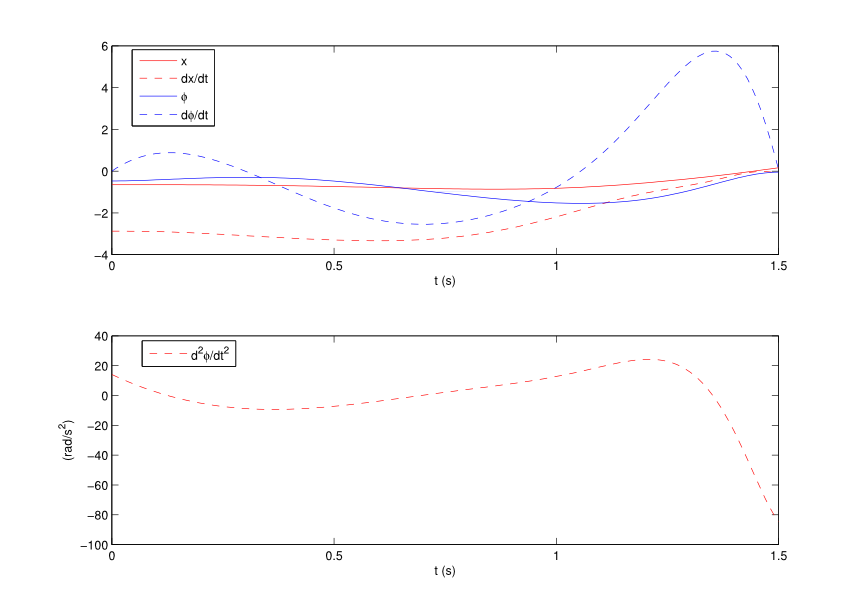
\includegraphics[width=\textwidth]{ballbeammatlab}
\caption{Example of trajectory generated using the gradient based iterative optimization. The states are plotted as deviations from the desired terminal condition. The second derivative of the angular velocity of the beam is used as control signal in this example, that that could easily be recalculated to the force required by the controller using the model.}
\label{fig:matlabtrajectory}
\end{figure}


\end{document}



